\documentclass[a4paper]{jpconf}

\usepackage{graphicx}

\usepackage{lineno}

\begin{document}

\title{DAQExpert - An expert system to increase CMS data-taking efficiency}

\author{J-M Andre\textsuperscript{5}, U Behrens\textsuperscript{1}, J Branson\textsuperscript{4}, O Chaze\textsuperscript{2}, S Cittolin\textsuperscript{4}, C~Contescu\textsuperscript{5}, G-L Darlea\textsuperscript{6}, C Deldicque\textsuperscript{2}, Z Demiragli\textsuperscript{6}, M Dobson\textsuperscript{2}, N~Doualot\textsuperscript{5}, S Erhan\textsuperscript{3}, J R Fulcher\textsuperscript{2}, D~Gigi\textsuperscript{2}, M Gladki\textsuperscript{2}, F Glege\textsuperscript{2}, G~Gomez-Ceballos\textsuperscript{6}, J~Hegeman\textsuperscript{2}, A Holzner\textsuperscript{4}, M Janulis\textsuperscript{2,a}, M~Lettrich\textsuperscript{2}, F~Meijers\textsuperscript{2}, E Meschi\textsuperscript{2}, R K Mommsen\textsuperscript{5}, S Morovic\textsuperscript{2}, V~O'Dell\textsuperscript{5}, S J Orn\textsuperscript{2}, L Orsini\textsuperscript{2}, I Papakrivopoulos\textsuperscript{7}, C Paus\textsuperscript{6}, P~Petrova\textsuperscript{2}, A Petrucci\textsuperscript{8}, M Pieri\textsuperscript{4}, D Rabady\textsuperscript{2}, A~Racz\textsuperscript{2}, T Reis\textsuperscript{2}, H~Sakulin\textsuperscript{2}, C Schwick\textsuperscript{2}, D Simelevicius\textsuperscript{2,a}, M Vougioukas\textsuperscript{2} and~P~Zejdl\textsuperscript{5,2}}

\address{\textsuperscript{1} DESY, Hamburg, Germany}
\address{\textsuperscript{2} CERN, Geneva, Switzerland}
\address{\textsuperscript{3} University of California, Los Angeles, Los Angeles, California, USA}
\address{\textsuperscript{4} University of California, San Diego, San Diego, California, USA}
\address{\textsuperscript{5} FNAL, Chicago, Illinois, USA}
\address{\textsuperscript{6} Massachusetts Institute of Technology, Cambridge, Massachusetts, USA}
\address{\textsuperscript{7} Technical University of Athens, Athens, Greece}
\address{\textsuperscript{8} Rice University, Houston, Texas, USA}
\address{\textsuperscript{a} Also at Vilnius University, Vilnius, Lithuania}

\ead{maciej.gladki@cern.ch}


\begin{abstract}
The efficiency of the Data Acquisition (DAQ) of the Compact Muon Solenoid (CMS) experiment for LHC Run 2 is constantly being improved. A~significant factor affecting the data taking efficiency is the experience of the DAQ operator. One of the main responsibilities of the DAQ operator is to carry out the proper recovery procedure in case of failure of data-taking. At the start of Run 2, understanding the problem and finding the right remedy could take a considerable amount of time (up to many minutes). Operators heavily relied on the support of on-call experts, also outside working hours. Wrong decisions due to time pressure sometimes lead to an additional overhead in recovery time. To increase the efficiency of CMS data-taking we developed a new expert system, the DAQExpert, which provides shifters with optimal recovery suggestions instantly when a failure occurs. DAQExpert is a~web application analyzing frequently updating monitoring data from all DAQ components and identifying problems based on expert knowledge expressed in small, independent logic-modules written in Java. Its results are presented in real-time in the control room via a~web-based GUI and a sound-system in a form of short description of the current failure, and steps to recover.
\end{abstract}

\section{Introduction}
The data-taking efficiency of the Compact Muon Solenoid (CMS) \cite{cms} experiment at CERN in 2016 during proton-proton physics, understood as the ratio of recorded over delivered luminosity, was 92.7\%, according to Web Based Monitoring (WBM). One of the major roles in operation is played by the Data Acquisition (DAQ) system, which controls the detector readout, event-building and operations of the event filtering farm \cite{daq}. The smooth operation of the experiment and its resulting high efficiency are ensured through constant supervision by a crew of operators and experts.

Being able to act within seconds during operations of LHC is one of the challenges of the operator. In order to simplify the operation of the complex DAQ system several tools exist to automate certain operations such as starting and stopping a run, configuring detector hardware and ensuring proper synchronization etc.\cite{assistance}. These tools facilitate the actions initiated by operators. However, it is not uncommon that the system goes into erroneous states where deeper understanding of the system is required to solve the problem in an optimal way. Experts of all subsystems prepare recovery instructions needed to resume data taking in an optimal way and as quickly as possible. Operators need to effectively select and execute them to make sure CMS operates smoothly.

Over the course of the last few years the list of recovery instructions became larger and more complex. Despite its straightforward form, it takes considerable time for the operator to find the correct remedy when needed. This part of the intervention, the reaction time, defined as the time between the problem occurrence and the start of the corresponding recovery action, is one of two concerns. Wrong or suboptimal decisions were not uncommon. These led to increased recovery time, defined as the time elapsed from the beginning of the recovery action to the resuming of data taking. The sum of the reaction and recovery time are referred to as the intervention time.

Reducing the reaction time and selecting the optimal recovery action are the two areas for improvement that will reduce the overall intervention time and directly affect the efficiency of CMS. We also aim to facilitate the post mortem analysis for human DAQ experts, to aggregate and to report a statistical analysis of the performance of the system and to reduce the need for external help especially outside of working hours without a deterioration of CMS efficiency. In order to achieve these goals we have developed a new expert system, the DAQExpert. It completely replaces the Perl based DAQ Doctor \cite{daqdoctor} which addressed these issues in the Run 1 DAQ system, but which only had rudimentary functionalities for the Run 2 DAQ system.

\subsection{Selecting the optimal recovery action}
The time spent recovering is the main contributor to the overall intervention time in CMS and amounts to 82\%. Therefore, it is essential to define and select the quickest set of actions needed to bring the system back to operation. Many different recovery procedures may be distinguished, e.g.: stopping and starting a run, (re)configuring and (re)initializing a specific subsystem, sending resynchronization or hard reset commands through the Timing Trigger and Control (TTC) system. They differ significantly in terms of impact they have on the system and how much time they take to complete. Some of them take a few seconds whereas others last for minutes. A common operator mistake is to issue the most general recovery procedure which solves most types of problems but takes longest time instead of using a faster problem specific action. DAQExpert was designed to help the operator make optimal decisions.

\subsection{Reaction time} \label{reaction-section}
The second area to improve is the time between occurrence of the problem and the first recovery action. There are sound notifications in the control room to draw the attention of the shifter when data flow stops. Identification of the problem and selecting the recovery action takes from a few seconds up to some minutes. We define the {\it comparison period} as the period of six months of data-taking (August 2016 - July 2017, excluding the Year End Technical Stop that lasted from December 2016 to April 2016, the month of May of 2017 was excluded due to special conditions of data-taking). Figure~\ref{reaction-histogram} shows the histogram of a reaction time for {\it comparison period}. Most of the times the operator reacted within 20-30 seconds. The aim of the project is to reduce the reaction time.


\subsection{Facilitating post mortem analysis}
Numerous monitoring systems enable access to data necessary to analyze the problem, albeit with some caveats. Some data are available after the problem has been resolved, some only while the problem is ongoing. In many cases some insight can be gained from the monitoring data on how to avoid similar problems in the future. The aim of the project is also to streamline the post mortem analysis by making both historic and real-time data easily available in the same way at any moment.



\section{Expert system and architecture}

The system consists of three services. Firstly, the {\it Snapshot Service} aggregates all monitoring information into a snapshot and persists it. Secondly, the { \it Reasoning Service} applies the knowledge of the experts on the snapshots. Finally, the { \it Notification Manager } manages and delivers notifications, including e-mail and live suggestions and sound notifications in the control room. The { \it DAQExpert } brings all parts together in the form of a web application enabling browsing of the whole history of monitoring data to view the analysis and to manage notifications. The design of the {\it Reasoning Services} and technologies used were driven by external forces.

\subsection{External forces}
The project's lifetime is expected to be up to 2024 and different developers will maintain it. Thus, one of the main constraints was to avoid short-lived and highly specific technologies which would make it difficult for new team members to quickly become productive. It needs to be easy to understand and modifiable, requiring little effort to learn. Rule-based engines have beed evaluated in the past by the CMS DAQ group and were considered unsuitable due to their steep learning curve. Introducing an additional programming language was not an option. The solution needed to be based on the current skill set of the team members and as simple as possible.

Moreover, the nature of the project foresees frequent logic-related updates, possibly introduced by many authors. Whenever a new recovery solution is advised by sub-system experts the corresponding knowledge needs to be introduced into the system. Finally, high availability is essential, as downtime of the system implies lack of support for the operators and possibly extended downtime of CMS. 

As a result, the new expert framework has been designed from the ground up. It allows to define the knowledge in imperative language popular in the group - Java. The knowledge is organized in small independent Logic Modules that are building blocks of the system.


\begin{figure}[h]
\begin{minipage}{18pc}
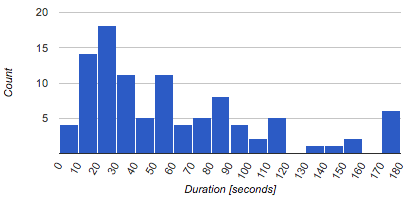
\includegraphics[width=18pc]{reaction-histogram-2016.png}
\caption{\label{reaction-histogram}Reaction time histogram.}
\end{minipage}\hspace{2pc}%
\begin{minipage}{18pc}
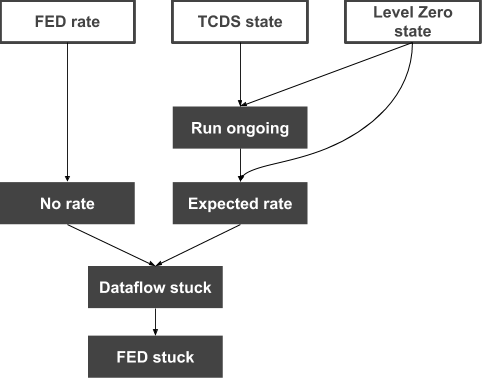
\includegraphics[width=18pc]{logic-module-hierarchy.png}
\caption{\label{subsetoflm}Subset of Logic Module hierarchy (white - observed parameters, blue - LM). }
\end{minipage} 
\end{figure}


\subsection{Monitoring, aggregation and data flow}

Multiple steps are needed before information from data sources is made available to the users. The monitoring data sources are queried to get information about data taking health. Monitoring data is collected from multiple heterogenous sources. They differ in terms of resolution, latency and time to retrieve. Diagnosing the problems of the data flow in real time requires quick access to key information. Post mortem analysis requires access to all relevant data at any time. To enable both, a so-called snapshot of the system is taken periodically, approximately every 2 seconds. It contains all necessary information to identify and understand the problem. Thus, the first step was to aggregate all the information in snapshots that bring together both structural data and instantaneous states of all components. The scope of the snapshot has been designed to give the full picture of the system's state at a given moment. Both real-time and post-mortem analysis are based on the same data from the snapshots.

While the snapshot is persisted for possible post-mortem analysis, it is simultaneously sent to the {\it Reasoning Service} for real time analysis. Notifications may result from the analysis and will be dispatched by the {\it Notification Service} and delivered to the clients.


\subsection{Implementation of expert knowledge}
It is common in the industry that the expert knowledge is defined in a declarative language. For instance, in a form of if-then-else rules expressed in a high-level rule-based language. As a result of external forces, this way of defining knowledge has not been used. A new custom made framework based on {\it Logic Modules} has been developed. A {\it Logic Module} (LM) is a~building block of {\it DAQExpert} logic. Each LM focuses on one specific aspect of the behaviour of the DAQ system:


\begin{itemize}
\itemsep0em
\item each LM defines one condition,
\item the definition of the condition is placed in the {\tt satisfy} method,
\item this method returns true if condition is satisfied and false otherwise,
\item one LM can use results of other LMs.
\end{itemize}

The knowledge defined in the LMs is used to find the optimal solution when a problem occurs in the data-flow. LMs operate on the snapshot and verify that key indicators and metrics are in expected states and within their specified ranges. As LMs may use outputs of other LMs, there is a predefined order of firing them. Figure~\ref{subsetoflm} presents a subset of LMs responsible for identifying one of many problems that may occur during data-taking. In the example there are five LMs and three parameters being monitored. The LMs are fired in top-down order allowing LMs to rely on others as indicated by arrows.


A LM may play two roles: it might be a sub-step of the analysis ({\it Expected rate}, {\it No rate}, {\it Dataflow stuck}) or final step of the analysis ({\it Front End Driver (FED) stuck}) delivering a description of the condition and a recovery suggestion. In the example shown in Figure~\ref{subsetoflm}, the following chain of LM was activated::

\begin{itemize}
\item {\it Run ongoing} -  data taking was active according to the {\it TCDS state} (TCDS - Timing and Control Distribution System) and{ \it Level Zero state} (Level Zero - Top level node in the run control system),
\item{\it No rate} - the average {\it FED rate} was 0, there was no data flowing
\item{\it Expected rate} - the {\it TCDS state}  and {\it Level Zero state} indicate that no recovery action is being issued at the moment, a run is ongoing according to output of {\it Run ongoing} LM and the readout rate is expected to be non-zero.
\item {\it Dataflow stuck} - this summarizes outputs of two LMs: {\it No rate} and {\it Expected rate}, and returns true if both are asserted, meaning that the data-flow is stuck,
\item {\it FED stuck} - starts the analysis when the {\it Dataflow stuck} condition is found. It performs specific checks to find the FED(s) which caused the data flow to stop. This LM identifies the problem precisely thus it contains instructions for the operator, including a detailed description of the problem and a recovery suggestion.
\end{itemize}



\section{Results}

The current version of the service improves all of the outlined areas. Operators of the DAQ system at CMS now have a tool delivering recovery action suggestions in real-time - the Dashboard (see figure~\ref{dashboard-tool}) at their disposal. Whenever a problem occurs the tool shows the description of the problem and the optimal steps to recover. It helps shifters to take correct decisions, reducing both reaction time and need of external human expert help.

Measuring the success of the project is quite a challenging task. The ultimate goal is to increase the data taking efficiency at the CMS. However, the overall efficiency is not an adequate figure of merit as it depends on many factors in addition to the quality of the DAQExpert suggestions. The detector is constantly being improved, there were major upgrades in both hardware and software which affected the final data taking efficiency of CMS. Feedback of operators and human experts is important as they are the target user groups of the system. As much as they appreciate the new system, the subjective verbal feedback cannot be used as a measure of success as it is not quantitive. Three parameters have been identified to adequately represent the success of the project: accuracy of the recovery action selection, reaction time of the operators and requests for external help. These are practically independent from other factors, which makes them a reliable means of comparison.

The DAQExpert was introduced in mid 2016, but operators were only instructed to use it in early 2017. All comparisons are based on {\it comparison period} (see section \ref{reaction-section}), corresponding to four months in 2016 without {\it DAQExpert} support and two months from 2017 where support was available. 


\subsection{Intervention time}

Improvement was mostly observed in the number of optimal recovery decisions taken by operators in case of data-flow interruptions. As stated before, the recovery time is the majority of the total intervention time (82\%), thus it is essential to minimize it by choosing the most appropriate and time-efficient recovery actions (optimal recovery actions). 

There are two main categories of recovery actions: heavy - lasting usually for 3-4 minutes, initiated by e.g. stopping the run; and light - lasting 7-10 seconds implemented with commands through the TTC system. Suboptimal decisions mean unnecessary time spent on recovery or irrelevant actions that will not solve the problem leading to similar problematic condition after its completion. On average this means that each suboptimal decision adds between 93 and 125 seconds of overhead to the recovery time.

In 2016, during data-taking, operators had no automatic guidance and out of 36 data-taking failures that were diagnosed by the DAQExpert, 32 times the optimal decision was taken. In 2017 there were 29 data-taking failures and all of the decisions were optimal.

The reaction time is a secondary metric to improve, as it is a minor (18\%) part of the total intervention time. There is a large variation depending on individual operator experience. The reaction time has slightly improved from 67 seconds in 2016 to 60 seconds in 2017. This is an area where the human factor plays an important role and bypassing the operators will certainly yield better results.


\begin{figure}[h]
\begin{minipage}{18pc}
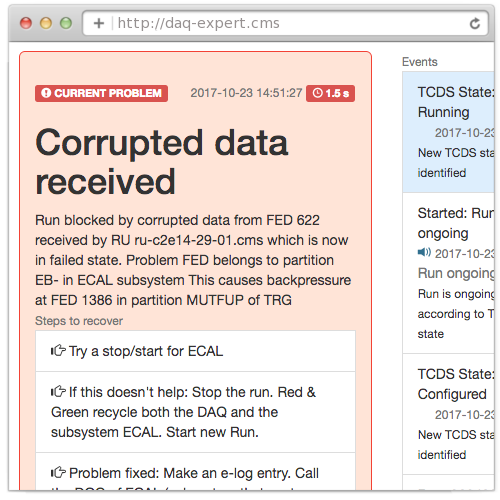
\includegraphics[width=18pc]{tool-dashboard.png}
\caption{\label{dashboard-tool}Dashboard - tool to show suggestions in real time.}
\end{minipage} \hspace{2pc}%
\begin{minipage}{18pc}
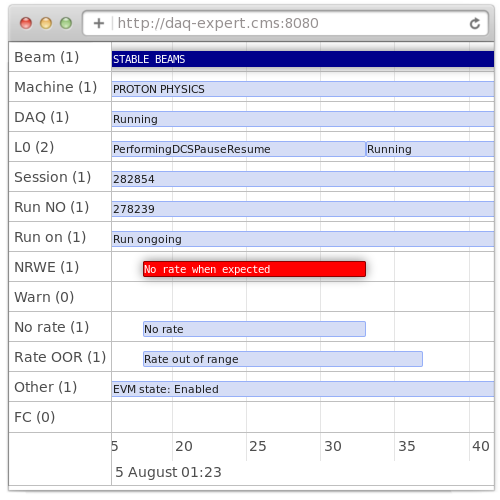
\includegraphics[width=18pc]{tool-browser2.png}
\caption{\label{browser-tool}Browser - tool to browse time evolution and to enable post mortem analysis.}
\end{minipage}
\end{figure}

\subsection{Non-quantitative results}
An improvement in the post-mortem analysis has also been made. In the case of more demanding data-flow interruptions, where further investigation is required, the{ \it DAQExpert} streamlines the chores of human experts. First, the go-back in time functions have been introduced that enable human experts to access the historic data easily with the timeline view ({\it Browser}), shown in figure~\ref {browser-tool}. Secondly, there are more data available to support post-mortem analysis than ever before. All monitored quantities of the system are kept for some period of time for debugging purposes.

\subsection{Summary}
Both quantitative and qualitative results on the launching of the new system were presented in this report. The recovery action selection accuracy was improved by introducing the expert system. There were no non-optimal recovery decisions observed after deployment of {\it DAQExpert}, whereas, before they occurred 11\% of the time. Additionally the average reaction time shrunk from 67 to 60 seconds, which means that the total intervention time, including reaction time and recovery procedure time, has been reduced by at least 10 seconds. One major improvement to be implemented in the future is to bypass the operator whenever possible. This will shorten the reaction time to a few seconds.
External help demand has not yet been quantified. This area is of great interest for on-call human experts as it has the potential to reduce their workload. The number of phone calls (normalized by the number of problems) to the on-call experts before and after {\it DAQExpert} introduction may reveal trends in this area.


\section*{References}
\begin{thebibliography}{9}

\bibitem{cms} CMS Collaboration 2008 {\it The CMS experiment at the CERN LHC} JINST 3 S08004
\bibitem{daq} Andre~J~M {\it et al} 2016 Performance of the new DAQ system of the CMS experiment for run-2 {\it Proc., 20th IEEE-NPSS Real Time Conf. (RT2016), Padua, Itally June 5-10, 2016}
\bibitem{assistance} Andre~J~M {\it et al} 2017 New operator assistance features in the CMS Run Control System {\it 22nd Int. Conf. on Computing in High Energy and Nuclear Physics, CHEP 2016, San Francisco, Usa, 10-14 Oct 2016}
\bibitem{daqdoctor} Bauer~G {\it et al} 2014 Automating the CMS DAQ {\it J. Phys.: Conf. Ser.} 513 012031
\end{thebibliography}





\end{document}


